\documentclass[12pt, a4paper, oneside]{ctexart}
\usepackage{amsmath, amsthm, amssymb, bm, color, framed, graphicx, hyperref, mathrsfs}

\title{\textbf{力学A(L) 2025秋 USTC}}
\author{姓名:石泊远$ \hspace{1cm} $学号:PB25000051}
\date{\today}
\linespread{1.5}
\definecolor{shadecolor}{RGB}{241, 241, 255}
\newcounter{problemname}
\newenvironment{problem}{\begin{shaded}\stepcounter{problemname}\par\noindent\textbf{Assignments ~ \arabic{problemname}. }}{\end{shaded}\par}
\newenvironment{solution}{\par\noindent\textbf{Solution. }}{\par}
\newenvironment{note}{\par\noindent\textbf{Assignments ~ \arabic{problemname}'s Remark. }}{\par}
\newenvironment{remark}{\noindent \textbf{Remark.}}{}

\begin{document}
	%Introduction
	\maketitle
	
	\begin{solution}
		a.$ \bm{A} + \bm{B} = ( 7,-2,9 )$ \\
		b.$ \bm{A} - \bm{B} = ( -3,-4,5 ) $ \\
		c.$ \bm{A} \cdot \bm{B} = 21 $ \\
		d.$ \bm{A} \times \bm{B} = ( -13,31,17 ) $
	\end{solution}
	
	\begin{solution}
		\begin{figure}[h]
			\centering
			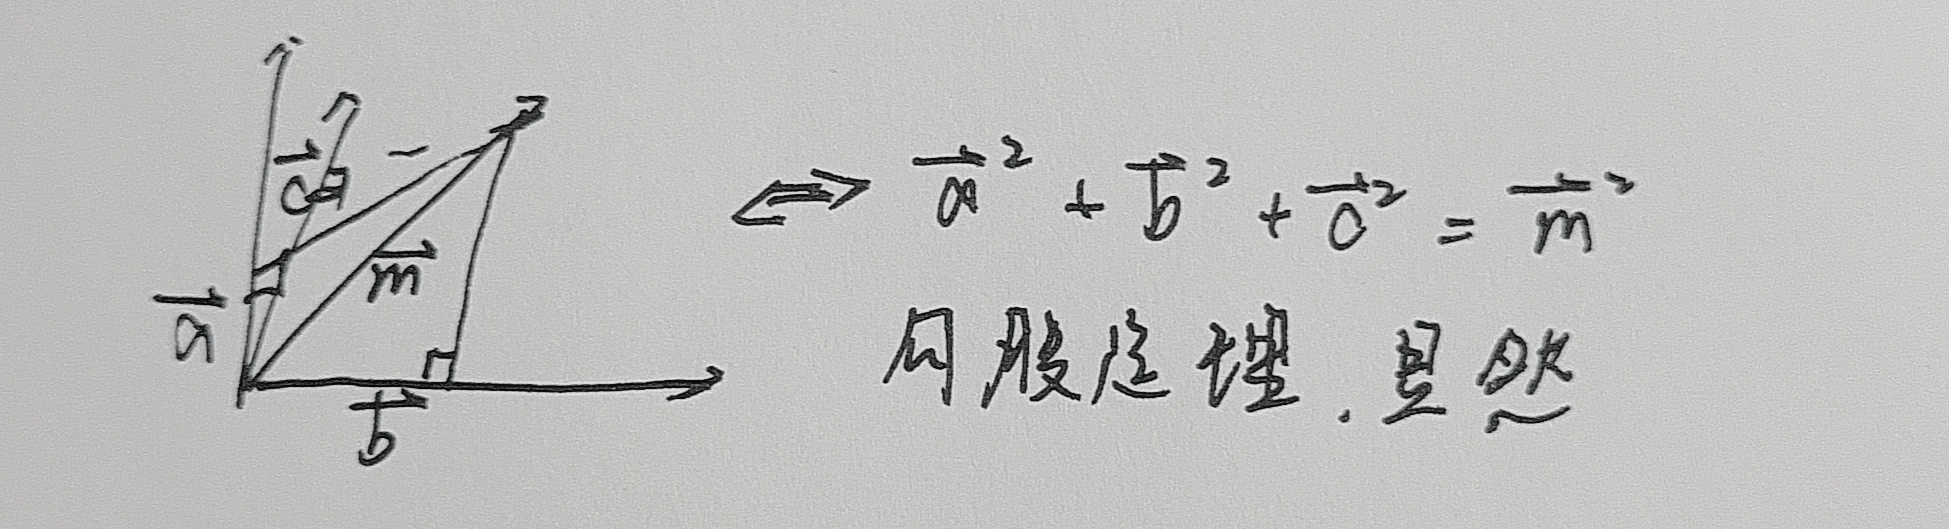
\includegraphics[width=0.7\textwidth]{72A71686E54C3E9870F55C330E117C8B.png}
		\end{figure}
	\end{solution}
	
	\begin{solution}
		\begin{figure}[h]
			\centering
			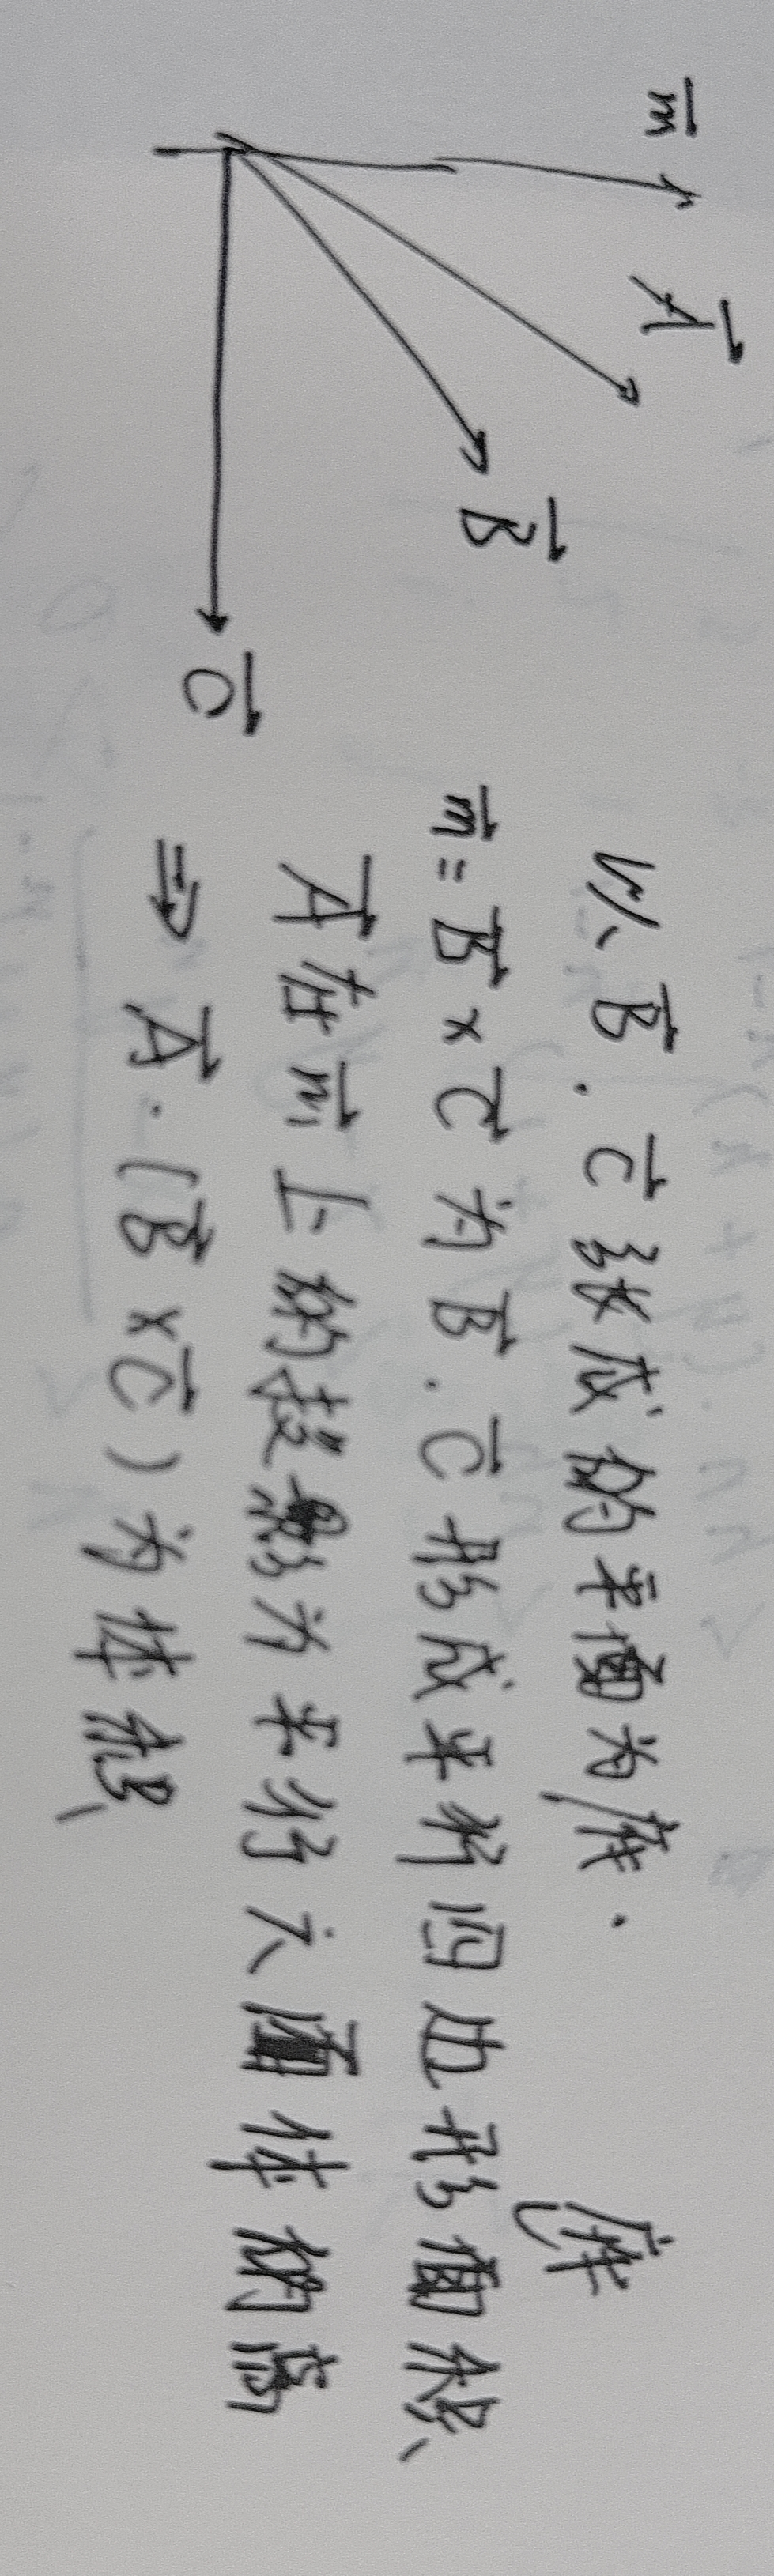
\includegraphics[scale = 0.09,angle=90]{3DBEE0976199DBEFBAC2BAE8C3F9E300.png}
		\end{figure}
	\end{solution}
	
	\begin{solution}
		第一项是在那个单位矢量上的分量,第二项是垂直方向的分量
	\end{solution}
	
	\begin{solution}
		$$ \Delta h = \dfrac{1}{2}g \Delta \left( t^2 \right) = \dfrac{1}{2}g \times \left( \left(\dfrac{T_A}{2} \right)^2 - \left(\dfrac{T_B}{2} \right)^2 \right) $$
		整理即得
	\end{solution}
\end{document}